\section{Introducción}

\vspace{0.5cm}

\Large\scshape
\begin{center}
    Contexto global e investigativo para la realización del proyecto
\end{center}
\normalfont

\divider

El precipitado incremento de la población mundial en las últimas décadas, causado por el acelerado desarrollo tecnológico humano a partir de mediados del siglo XX, ha generado un exponencial aumento de demanda energética para poder satisfacer los constantemente crecientes requerimientos de la población. En respuesta a esta incrementada demanda del sistema energético mundial, los países comenzaron a crecer su capacidad instalada de plantas de generación en base a la quema de combustibles fósiles (petróleo, carbón, gas, etc.), sin tener en cuenta el catastrófico impacto que tienen sobre la biósfera terrestre sus grandes emisiones de gases de efecto invernadero, como dióxido de carbono y metano.\\

Hoy en día, más de medio siglo después, las consecuencias de este desmedido incremento del consumo global de combustibles fósiles se pueden observar claramente en la temperatura promedio del aire superficial de la Tierra, que ya es más de 1°C mayor a temperaturas medidas a principio del siglo previo (figura \ref{Temp_Tierra})$^{[OWID-CO2AndGreenhouseEmissions]}$, con algunos estimados conservadores de más de 2.5°C para finales de siglo$^{[ref 12 Wikipedia]}$. Los efectos perjudiciales de este incremento de temperatura se pueden ver en muchas partes, como la extinción de especies, el retroceso de los glaciares, el aumento de incidencia e intensidad de fenómenos climatológicos extremos (tormentas, sequías, olas de calor, etc.), entre muchos otros.

\begin{figure}[H]
    \centering
    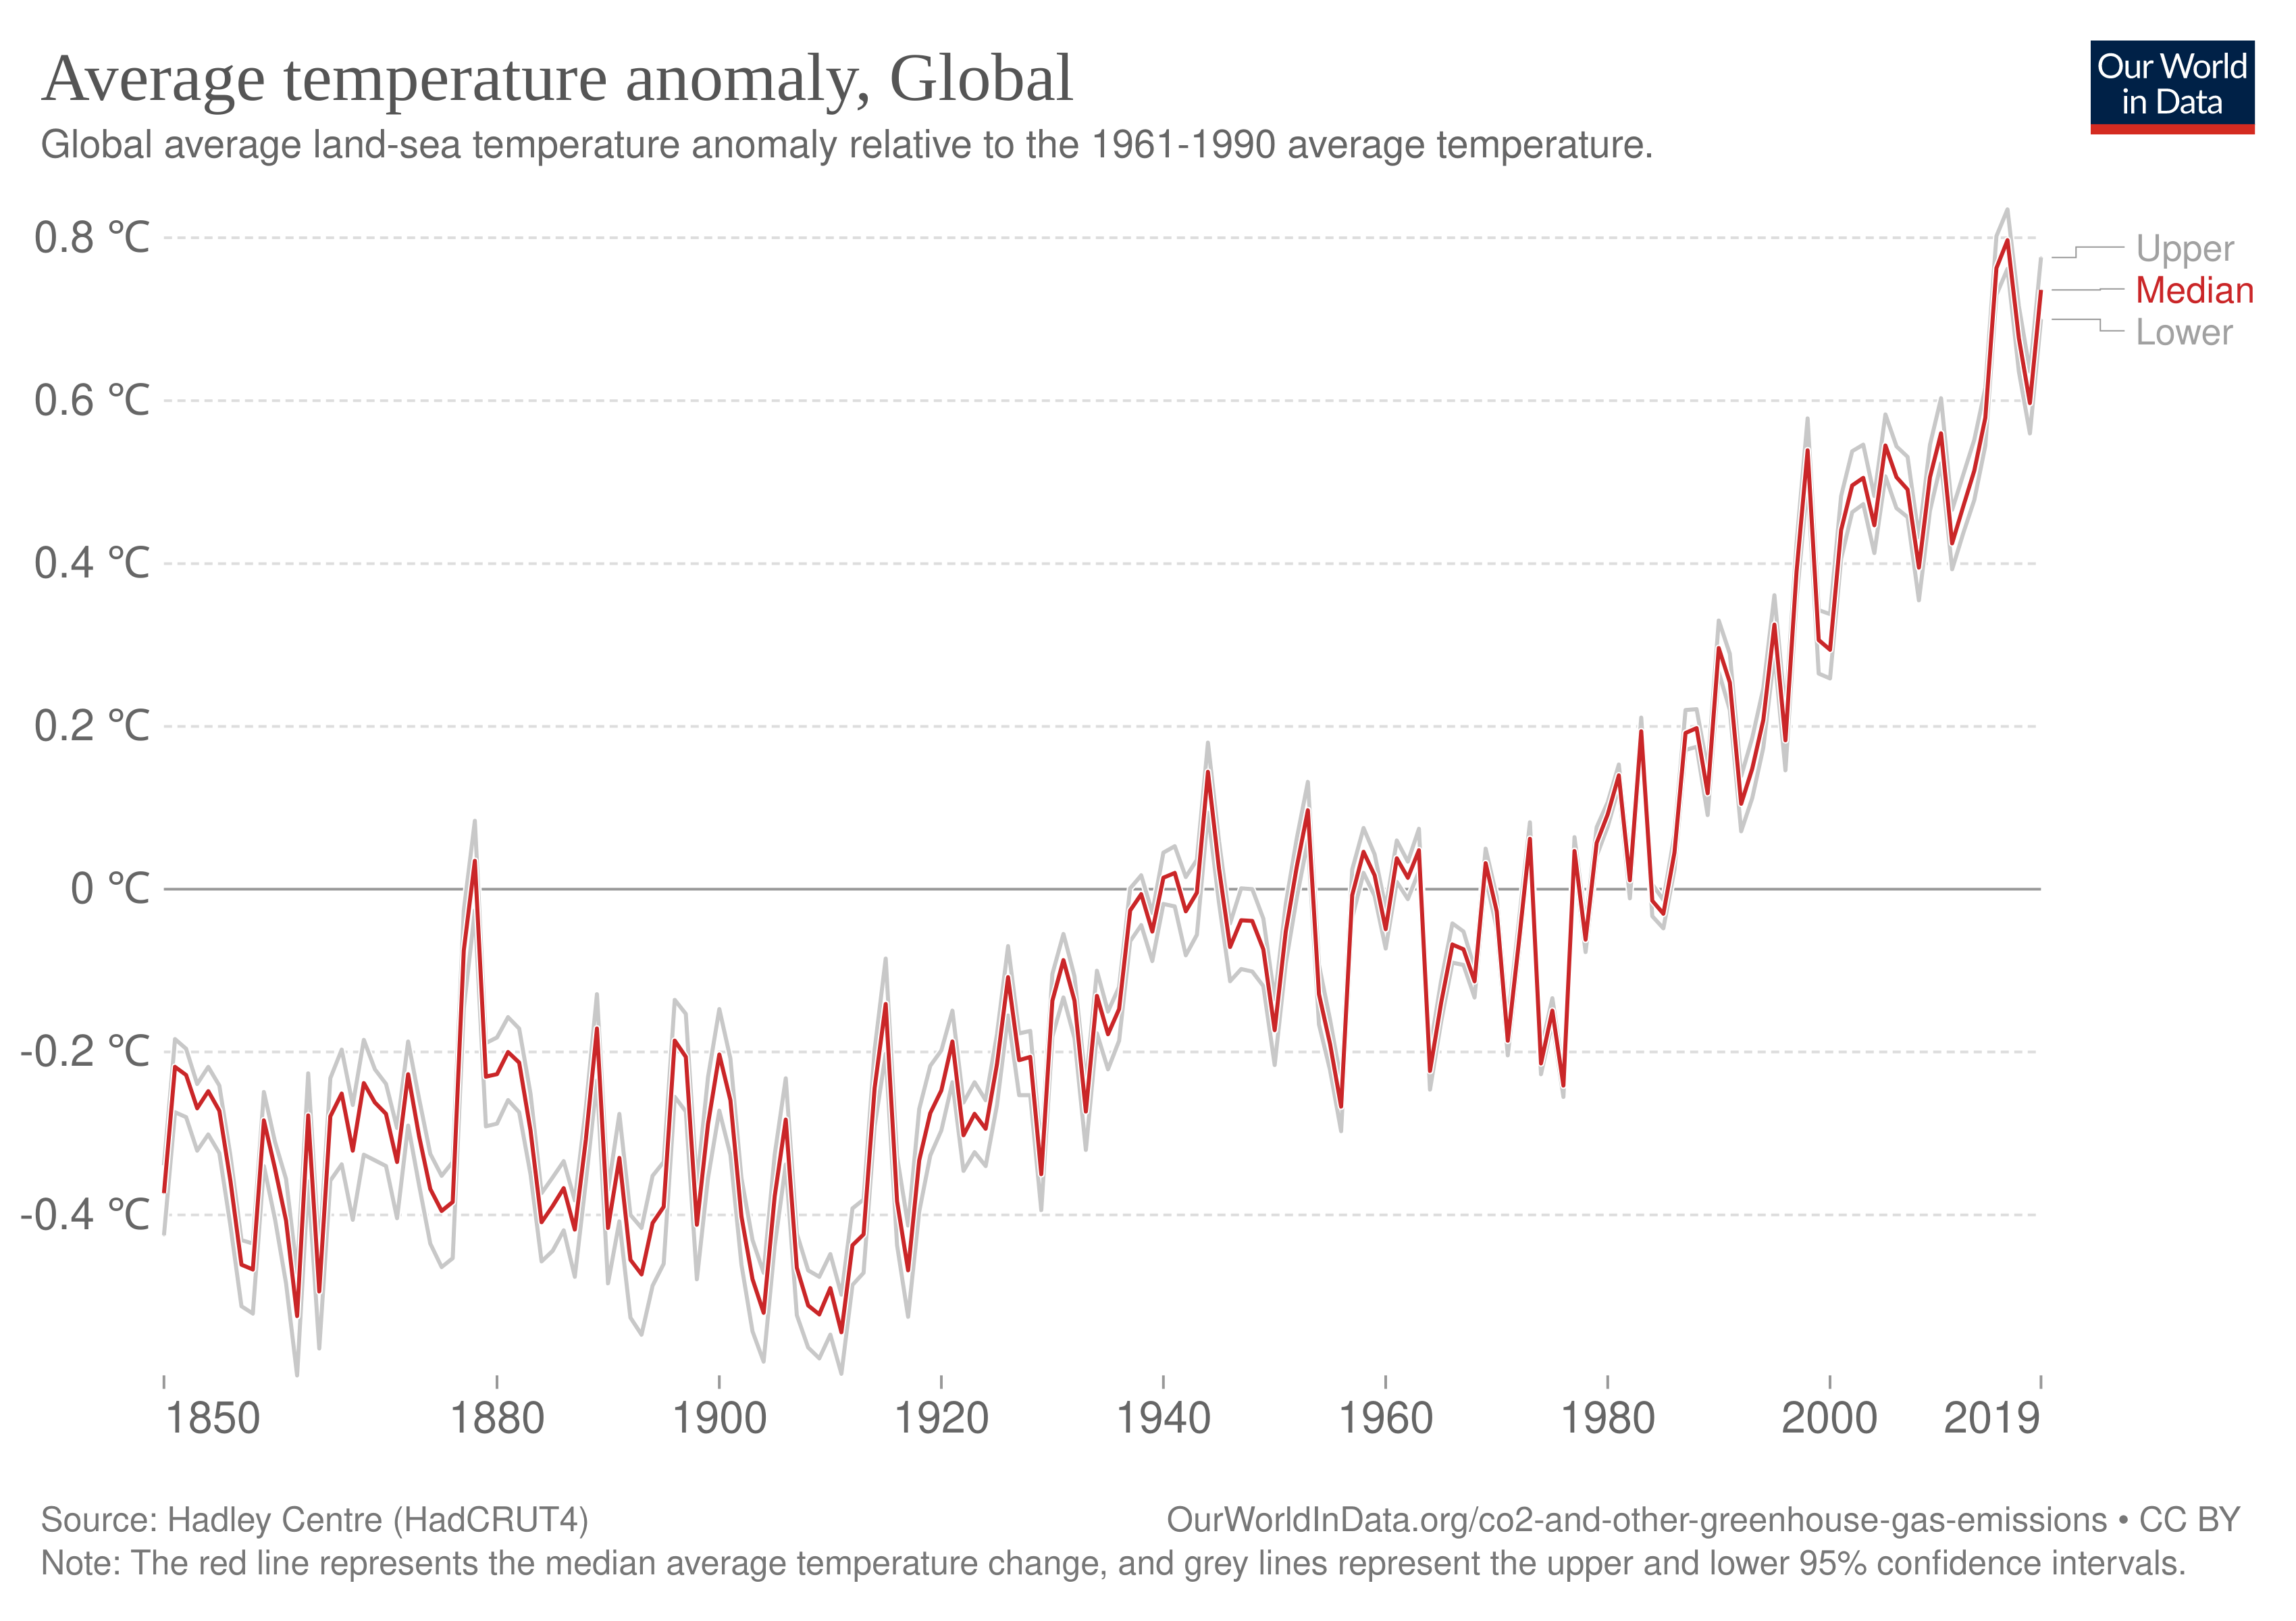
\includegraphics[scale=0.11]{Imagenes/Grafico Temperatura.png}
    \caption{Temperatura superficial promedio del planeta, relativo a la temperatura promedio de 1961-1990, desde 1850 hasta 2019.}
    \label{Temp_Tierra}
\end{figure}

Sin embargo, los combustibles fósiles y fuentes de energía no renovables siguen conformando una mayoría en el panorama de generación energética global: en el año 2019, alrededor del 85\% de la energía producida mundialmente provino de fuentes no renovables$^{[OWID-EnergyProduction]}$ (figura \ref{Emisiones_CO2}). Para frenar el avance del cambio climático, se debe acelerar el ritmo de adopción de energías alternativas como reemplazo de los combustibles fósiles, disminuyendo la emisión de CO$_2$ y metano en la atmósfera.

\begin{figure}[H]
    \centering
    \includegraphics[scale=0.11]{Imagenes/Grafico Fuentes de Energía.png}
    \caption{Distribución de producción global de energía según fuente, desde 1950 hasta 2019.}
    \label{Emisiones_CO2}
\end{figure}

Con esta motivación, el Instituto de Investigaciones en Electrónica, Control y Procesamiento de Señales (LEICI) de la Facultad de Ingeniería de la UNLP se embarcó en en proyecto ``Electrónica de Potencia y Sistemas de Control Avanzado Aplicados a Fuentes de Energía Alternativas'', dentro del cuál se enmarca el presente trabajo, que utiliza pilas de combustible a base de hidrógeno como fuente de energía alternativa.\\

La plataforma experimental para la evaluación de sistemas híbridos basados en pilas de combustible consiste de múltiples partes, que se detallan en la figura \ref{diag_plataforma} a continuación.

\begin{figure}[H]
    \centering
    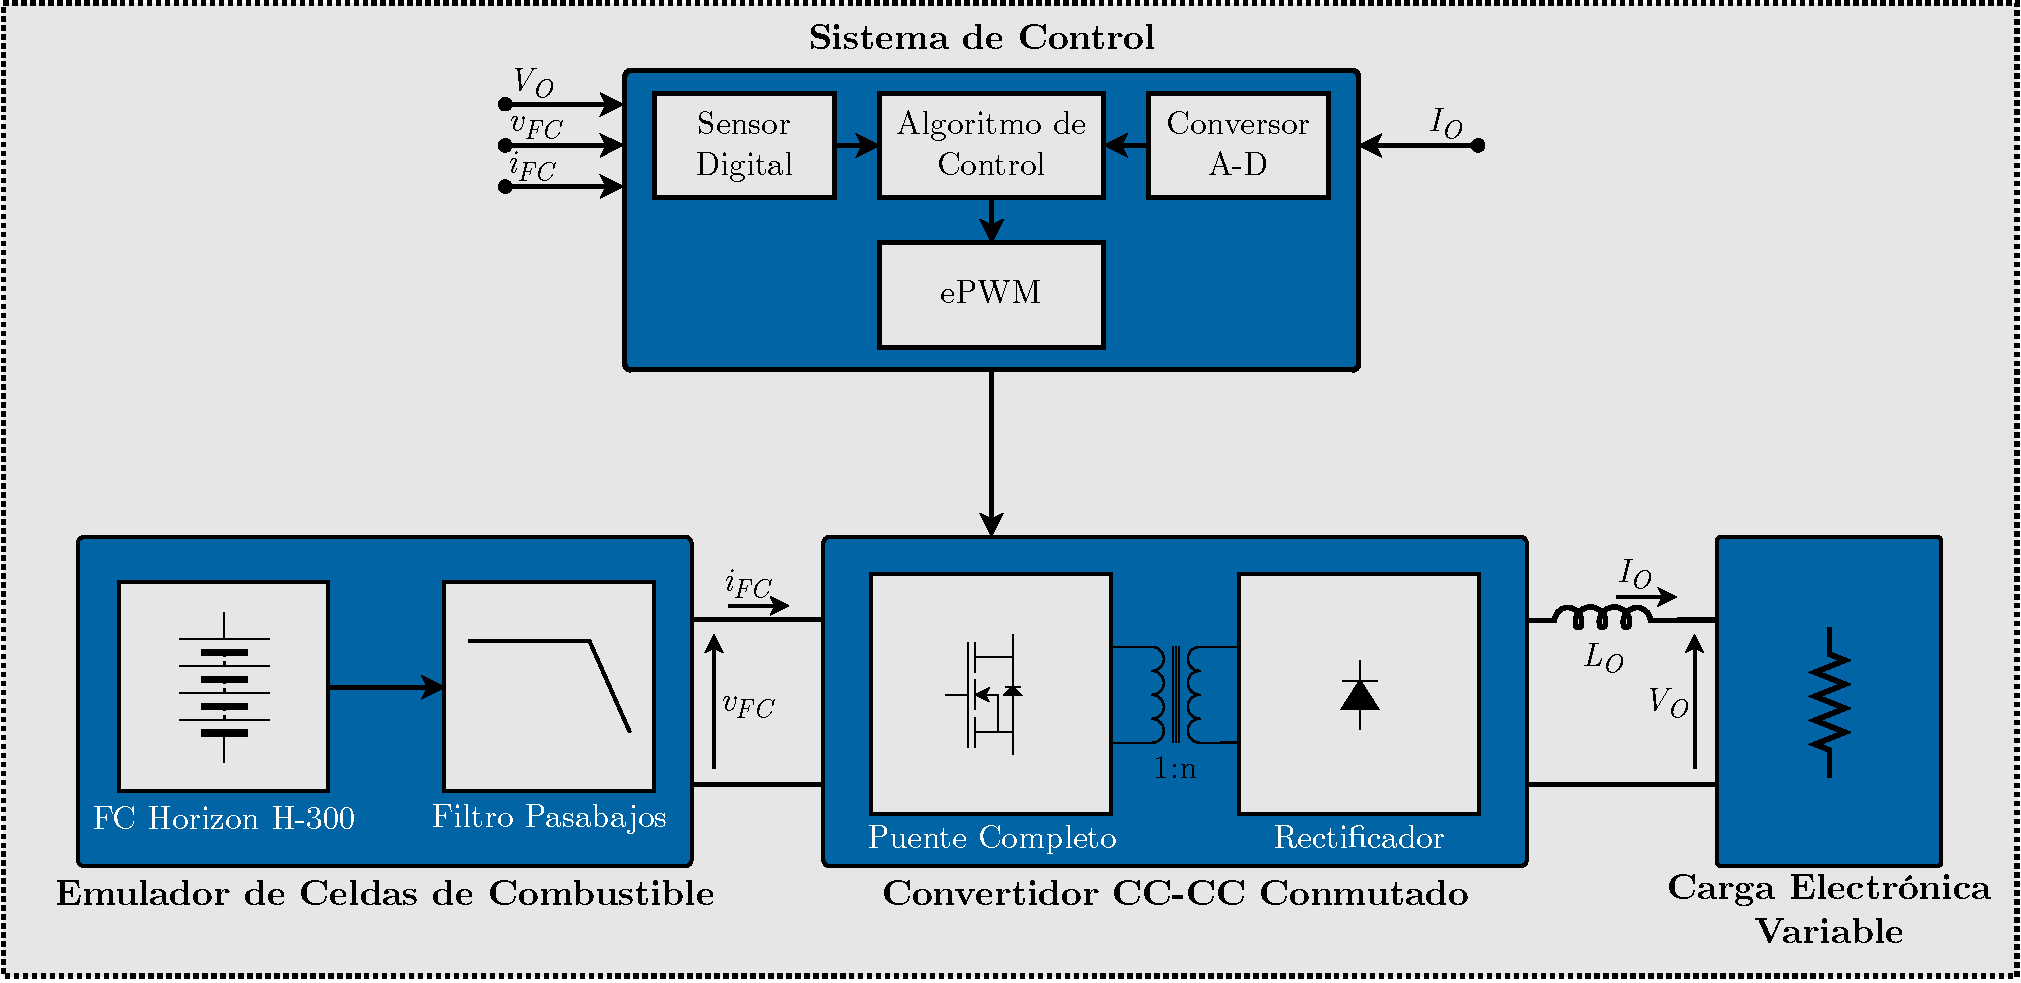
\includegraphics[scale=0.4]{Imagenes/Plataforma Experimental.pdf}
    \caption{Diagrama de la plataforma experimental en estudio.}
    \label{diag_plataforma}
\end{figure}



\subsection{Conversores CC-CC conmutados}

